\documentclass{article}

\usepackage[dblblindworkshop, final]{neurips_2026}

\workshoptitle{TAE (Trust-AI-Eval): Can We Trust AI Evaluation?}

\usepackage[utf8]{inputenc}   %
\usepackage[T1]{fontenc}      %
\usepackage{hyperref}         %
\usepackage{url}              %
\usepackage{booktabs}         %
\usepackage{amsfonts}         %
\usepackage{amsmath}          %
\usepackage{amsthm}           %
\usepackage{nicefrac}         %
\usepackage{microtype}        %
\usepackage{graphicx}         %
\usepackage{xcolor}           %

\raggedbottom
\setlength{\textfloatsep}{9pt plus 2pt minus 3pt}
\setlength{\floatsep}{9pt plus 2pt minus 3pt}
\setlength{\intextsep}{9pt plus 2pt minus 3pt}
\renewcommand{\topfraction}{0.92}
\renewcommand{\bottomfraction}{0.75}
\renewcommand{\textfraction}{0.08}
\renewcommand{\floatpagefraction}{0.75}

\setlength{\abovedisplayskip}{7pt plus 2pt minus 2pt}
\setlength{\belowdisplayskip}{7pt plus 2pt minus 2pt}
\setlength{\abovedisplayshortskip}{4pt plus 1pt minus 1pt}
\setlength{\belowdisplayshortskip}{4pt plus 1pt minus 1pt}

\newtheorem{definition}{Definition}
\newcommand{\mdi}{\mathrm{MDI}}
\newcommand{\fip}{\mathrm{FIP}}
\newcommand{\env}{\mathrm{env}}


\title{MDI: The Minimum Detectable Improvement of an LLM Judge}

\author{%
  Hyeong-seob Kim \\
  WIGTN \\
  \texttt{harrison@wigtn.com} \\
}

\begin{document}

\maketitle

\begin{abstract}
  Where a pipeline's outputs are closed, a golden dataset holds the yardstick
  still; open-output pipelines scored by an LLM judge have no such anchor:
  the same output scored twice does not, in general, receive the same score. We
  ask what improvement claims such a measurement can support, and define
  $\mdi(\env, N)$, the \emph{minimum detectable improvement}: the smallest gain
  an environment can confirm at a stated error level given $N$ scoring repeats,
  the half-width of the null distribution's 95\% prediction interval; and
  $\fip(\Delta, \env, N)$, the probability that an observed gain $\Delta$
  reverses under independent re-evaluation. On a grid of two
  judges, two tasks, and three scales we tabulate $\mdi$, the power (Type~II)
  side that acceptance testing leaves uncontrolled, over
  $N \in \{1,3,5,8,10\}$, where it spans $2.7\times$ across one judge tier at
  $N{=}1$; a repeat sweep separates instability-driven gains, which vanish as $N$
  grows, from a residue repeats cannot reach, which a decay model puts at a
  non-zero floor. That floor depends on the measurement's own design: widening the
  family of accepted rubric rewordings from four to eight raises it
  $2.5\times$ in variance while the repeat-reducible component holds.
  Against expert annotations the threshold fires on pairs no annotation facet
  separates and stays silent on one that three of four do: a measured
  boundary on what it licenses. We close with a
  reporting-and-decision protocol (repeat, interval, decide, with an SLA
  margin for absolute claims) that every number here obeys. The grid is
  pilot-scale: it establishes direction, leaving cell-level magnitudes to the
  expanded grid.
\end{abstract}

\section{Introduction}
\label{sec:introduction}

Where a pipeline's outputs are closed (classification labels, extraction
fields, retrieval hits), practice is settled: build a golden dataset, report
recall and precision, ship when the numbers clear the service threshold. A
golden dataset's real force is not that it stores correct answers but that it
holds the yardstick still: the same output scored twice gets the same
score. Open-output pipelines (agent transcripts, long-form generation, tool-use
traces) admit no such dataset; teams put an LLM judge in its place, and a judge
scoring the same output twice does not, in general, return the same number.
That is measured, not assumed: scored ten times over, several judges disagree
with themselves, and for most of them temperature zero does not settle it
\citep{lau2026sameinput}. This paper addresses the question that situation
forces: \emph{in open-output pipelines where no golden dataset can exist, what
licenses a verdict?}

\paragraph{Certify the instrument before trusting the reading.}
Before a factory trusts a gauge to accept or reject parts it measures how much
the gauge itself wobbles, and calls a part-to-part difference real only once it
exceeds that spread. We do the same for the LLM judge: measure its spread by
repeating it, and read a smallest resolvable difference off that. (Intuition
only; Section~\ref{sec:framework}'s definitions stand without it.)

Our answer is deliberately narrow. Failing our bar does not make a verdict
wrong; it breaks the link between the measurement and the claim, not the
judgment itself. A verdict far from its threshold survives an unsteady
yardstick; one near threshold, without margin, does not
(Section~\ref{sec:protocol} turns that margin into a table).
The lineage we borrow keeps two thresholds: detectable, and important
by an external criterion (Section~\ref{sec:related}); $\mdi$ is the first;
Contribution~5 measures the gap to the second.

We treat this as a problem of \emph{measurement rigor} in evaluation science,
and the field has asked for exactly that: \citet{bean2025construct} find only
$16\%$ of $445$ LLM benchmarks using uncertainty estimates or statistical
tests, \citet{apollo2024science} call for ``a science of evals,'' and
\citet{jiang2026itemlevel} want item-level results released rather than
discarded. We answer a small slice of it: the test--retest reliability of the
LLM judge, and what it implies for when an observed gain licenses a claim.

The acceptance side has begun to be addressed: a concurrent preprint
\citep{zayxshawn2026pace} gives an anytime-valid acceptance test for
accept-if-better rules and notes that its guarantee does not control
\emph{power}. That open side is what we take up. Type~I control asks whether a
claimed gain is real; we ask first whether the measurement can resolve a gain
of that size at all. This does not conflict with reinforcement
learning's tolerance of verifier noise \citep{plesner2026imperfect}: there
noise is redrawn each epoch and averaged over rollouts, while an
evaluation-gated pipeline sends the same noise through an accept-if-better
gate. Averaging cancels noise; selection amplifies it.

\begin{figure}[t]
  \centering
  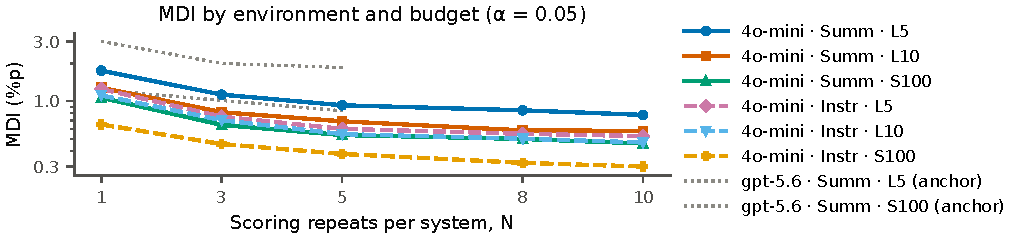
\includegraphics[width=\linewidth]{../figures/mdi_overlay_alpha0p05.pdf}
  \caption{The smallest gain an evaluation can separate from judge noise is not
    a constant: it depends on the environment ($2.7\times$ across the coloured
    dense tier at $N{=}1$) and on the budget $N$. Anchor curves (grey) use fewer
    items and repeats and are left out of that ratio; values in
    Table~\ref{tab:exp1-lookup}.}
  \label{fig:mdi-overview}
\end{figure}

\paragraph{Contributions.}
\begin{enumerate}
  \item \textbf{An $N$-dependent Minimum Detectable Improvement.} We
    formalize $\mdi(\env, N)$: a decision threshold expressed in observed
    score-difference units that is a function of the measurement budget $N$
    (scoring repeats). Prior work measures judge-level thresholds
    $\Delta^*(J)$ (cf.\ \citealp{usami2026darkcurrent}); where a repeat
    axis exists it counts calls to recover the judge's \emph{own} majority
    verdict \citep{yagubyan2026coinflip}; a detection threshold as a
    function of $(J, N)$ is unclaimed.
  \item \textbf{The False Improvement Probability, conditioned on the
    observed gain.} $\fip(\Delta, \env, N)$: the probability an observed
    gain $\Delta$ reverses under independent re-evaluation; conditioning
    on the \emph{observed} $\Delta$ is unclaimed in prior work.
  \item \textbf{A budget-indexed table of $\mdi$.} Per budget
    $N \in \{1,3,5,8,10\}$, the smallest gain each environment can separate
    from noise at level $\alpha$, with the stated multiplier to any target
    power, the Type~II side that acceptance testing leaves uncontrolled.
  \item \textbf{Noise-channel separation by a repeat sweep.} More scoring
    repeats make instability-driven gains vanish while a procedural
    component remains, which the sweep prices; clearing the threshold
    therefore rules out the instability channel alone, not judge bias
    (Section~\ref{sec:limitations}). We demonstrate the sweep on our grid
    and apply the promotion-time noise test it implies to a public
    improvement-loop trace released without repeats.
  \item \textbf{A measured boundary on what the threshold licenses.}
    Clearing $\mdi$ separates pairs on the judge's own scale while carrying
    almost no information about whether an expert reference agrees: it fires
    on pairs no annotation facet separates, and stays silent on one that
    three of four do (Section~\ref{sec:exp1}): the detectable/important
    pair's second threshold, measured rather than assumed.
\end{enumerate}

The measurements reported here are pilot-scale (direction, not final
precision), and every quantitative claim in the paper obeys the protocol it
proposes (Section~\ref{sec:protocol}).

\section{Related Work}
\label{sec:related}

Six clusters border this work; each full contrast is stated once, next to
the definition it qualifies (Section~\ref{sec:framework}), and this section
is the map. \emph{Error decomposition}: TEE \citep{messing2026tee}
decomposes total evaluation error across judges, prompts, and temperatures
via crossed random effects; we ask the downstream question (given that error, when is an improvement claim
licensed?) and consume their variance components as \emph{inputs}, a builds-on, consumed-not-replaced
relation. \emph{Resolution statistics}: the nearest priors to $\mdi$, Feuer et al.'s $\mathrm{Sens}$
\citep{feuer2025judgmentnoise} and the
per-response-pair detection threshold
$\Delta^*_{75}$ of \citet{usami2026darkcurrent}, describe the judge alone, with no repeat or
budget axis (full contrast after Definition~\ref{def:mdi}).
\emph{Item-axis detectability}: \citet{kotawala2026resolution} and
\citet{zhuang2026preregistering} ask how large a gain a benchmark can detect at
its item count; both treat items as the only noise source and assume a scorer
that gives the same answer twice.
\emph{Statistical lineage}: $\fip$ descends from Card et al.'s Type-S
error \citep{card2020power} and is the measurement-stage sibling of
Baumann et al.'s FDR conditioned on the observed $p$
\citep{baumann2025llmhacking} (contrast after Definition~\ref{def:fip}).
\emph{Loop-side thresholds}: VRR-Stop \citep{wu2026vrrstop} states its
accept threshold in optimizer units with $M{=}8$ verifier queries; ours is
in observed score-difference units, and our sweep includes $N{=}8$ so the
two are directly comparable (Section~\ref{sec:exp3}). \emph{Measurement theory and institutions}: of
the contested psychometrics import we take test--retest reliability only.
The construction of $\mdi$ is that of the smallest detectable difference of
classical test--retest theory ($1.96\sqrt{2}\,\mathrm{SEM}$, the half-width of
the null distribution of a re-measured difference
\citep{beckerman2001srd, weir2005sem}), carried from one subject to an item-set
mean and indexed by a measurement budget the clinical form has no analogue for.
That lineage never reads detectability alone: a change claim must also
clear a minimal \emph{important} difference against an external criterion
\citep{devet2006minimal, devet2011measurement}; we import the pair, and
Section~\ref{sec:exp1} measures the gap between them.
The classical frame is generalizability theory, whose D-study
\citep{cronbach1972dependability, brennan2001generalizability} already sizes
measurement conditions for a target dependability and whose variance
decomposition is Eq.~\ref{eq:decay}; \citet{song2025autoscoring} run that
D-study on LLM-scored essays. In their design a ``rater'' is a different model
and each model scores once, so they answer how many models to average. We ask
how many times to call one model, a facet their design cannot see. Our
delta is not estimation theory but the unit, the conditioning on the observed
$\Delta$, and $\sigma$, $\omega$ measured over that facet. The EU JRC lists failure to distinguish signal from
noise among the field's structural problems \citep{eriksson2025trust}, and
NIST AI 800-3 already requires repeat trials with valid confidence
intervals \citep{nist2026ai8003}, the frame we extend to a stochastic
scorer.

\section{Framework: MDI and FIP}
\label{sec:framework}

\paragraph{(i) A judge score is a draw from a distribution.}
Fix an evaluation environment
\begin{equation*}
  \env = (\text{judge model},\ \text{prompt template},\ \text{task},\
  \text{scale format},\ \text{temperature})
\end{equation*}
and an output $x$. The judge's score is not a constant of $(x, \env)$. Repeat
the same call $r = 1, \dots, N$ times and it returns draws $s^{(r)}(x;\env)$
from a distribution. Everything below follows from keeping that distribution
instead of using its first value. Scores are reported scale-normalized (\%p;
raw values in the appendix). We write $\bar{s}_N$ for a system's item-mean
score over $N$ repeats and $\Delta = \bar{s}_N^A - \bar{s}_N^B$ for the
observed gain.

\paragraph{(ii) $\sigma(\env)$ is observable only through same-input repeats.}
The spread $\sigma(\env)$ cannot be read off a single run, a leaderboard or a
model card: it is observable only by scoring the \emph{same input} repeatedly
in the \emph{same environment}. That is the one idea we take from psychometrics
(test--retest reliability), and Section~\ref{sec:experiments} is built to
produce such repeats.

\paragraph{(iii) The prediction interval of an observed gain.}
When the true gain is zero, the observed $\Delta = \bar{s}_N^A - \bar{s}_N^B$
still has a distribution, inherited from the judge's. Inside its central 95\%
prediction interval, a gain cannot be told apart from the judge scoring the
same thing again. That interval depends on $(\env, N)$ and not on which
systems are compared. Definition~\ref{def:mdi} states this as the null
distribution $D_0(\env, N)$, estimated nonparametrically from
repeated-scoring data.

\paragraph{(iv) $N$-dependence and the noise floor.}
The interval shrinks with the measurement budget $N$, but not to zero. The
variance of a mean of $N$ repeats decomposes as
\begin{equation}
  \label{eq:decay}
  \operatorname{Var}\!\left[\bar{s}_N\right]
    \;=\; \frac{\sigma^2(\env)}{N} \;+\; \omega^2(\env),
\end{equation}
the standard variance-components form (cf.\
\citealp{miller2024errorbars, messing2026tee}). Repeats reduce
$\sigma^2(\env)$; they do not touch the floor $\omega^2(\env)$. Two things
follow: the threshold depends on $N$, and buying more repeats stops paying at
$\omega(\env)$. Experiment~3's sweep fits Eq.~\eqref{eq:decay} per environment
to estimate both, and its $\omega^2$ independently replicates the CI
half-width floor of \citet{messing2026tee}.

\paragraph{(v) Everything depends on the environment.}
Every quantity above depends on $\env$. A threshold computed for one judge,
prompt, task, and scale does not carry over to another; the grid of
Section~\ref{sec:experiments} measures how badly it fails to carry over, which
is why every table is indexed by environment.
An environment includes the scoring harness (parsing, rubric rendering,
retries, provider), so in measurement-theory terms our intrinsic axis is
\emph{repeatability} and our procedural axis \emph{reproducibility}.

\paragraph{(vi) A procedure, not a benchmark.}
A fixed-item benchmark would contradict the thesis that every quantity here
depends on the environment. What we offer is the procedure a team runs to get
its own numbers, plus the implementation; the tables below illustrate it rather
than replace it.

\subsection{FIP and MDI}
\label{sec:framework-defs}

\begin{definition}[False Improvement Probability]
  \label{def:fip}
  For an observed gain $\Delta$ measured in environment $\env$ with $N$
  scoring repeats per system,
  \begin{equation*}
    \fip(\Delta, \env, N)
      \;=\; P\bigl(\Delta' \le 0 \,\big|\, \text{observed } \Delta,\ \env,\ N\bigr),
  \end{equation*}
  where $\Delta'$ is the gain re-measured under an independent replication
  in the same environment with the same budget. $\fip$ is estimated
  nonparametrically from repeated-scoring data (Experiment~2).
\end{definition}

Conditioning on the observed effect is the move \citet{baumann2025llmhacking}
make for annotation-stage $p$-values; we make it for measurement-stage
score gains. The ancestor of both is Card et al.'s Type-S error
\citep{card2020power}, with the stochasticity relocated from the sample to
the scorer.

\begin{definition}[Minimum Detectable Improvement]
  \label{def:mdi}
  Let $D_0(\env, N)$ be the distribution of mean score differences between
  two independent $N$-repeat scorings of the \emph{same} systems in
  environment $\env$ (pairs whose true skill difference is zero by
  construction). Then
  \begin{equation*}
    \mdi(\env, N)
      \;=\; \tfrac{1}{2}\,
      \operatorname{width}\!\bigl(\mathrm{PI}_{95\%}\bigl[D_0(\env, N)\bigr]\bigr),
  \end{equation*}
  the half-width of the central 95\% prediction interval of the null
  distribution. Via Eq.~\eqref{eq:decay}, $\mdi$ falls with $N$ at a rate
  set by $\sigma^2(\env)$ and flattens onto the floor $\omega(\env)$: the
  dependence on $N$ is part of the definition.
\end{definition}

$D_0$ is built by splitting each cell's estimation repeats, per item, into two
disjoint pools and collecting the difference of their $N$-repeat means
(Appendix~\ref{app:extra}).

We \emph{define} rather than derive $\mdi$, for a practical reason: the null
interval is exactly the region in which the instrument cannot tell two
identical systems apart. One property should be stated plainly: a true gain
of exactly $\mdi$ is measured above $\mdi$ only about half the time. So $\mdi$
controls false claims at the stated level $\alpha$, not the chance of catching a real gain.
A team that wants an $80\%$ chance needs a larger gain, and we measure the
factor rather than assume it: shifting $D_0$ and reading where $80\%$ of it
clears $\mdi$ gives $1.43\,\mdi$ (median over 36 cells, range
$1.34$--$1.46$; the closed-form cross-check is
Appendix~\ref{app:extra}). We tabulate the $\alpha$-level value
because $D_0$ measures it directly, and carry the $80\%$ column beside it.
The FIP-crossing read-off
$\min\{\Delta : \fip(\Delta, \env, N) \le \alpha\}$ is a consistency probe,
not a second definition; it sits \emph{above} the null-PI value and
Section~\ref{sec:experiments} reports the gap. Every decision here uses the
null-PI $\mdi$.

The nearest prior statistics describe the instrument, not the decision. Feuer
et al.'s $\mathrm{Sens}$ \citep{feuer2025judgmentnoise} carries no
$N$-dependence, and $\Delta^*_{75}$ of \citet{usami2026darkcurrent} is measured
per response pair from single calls: $\Delta^*(J)$, where $\mdi$ is $\Delta^*(J, N)$ at
a stated error level. The MDE lineage \citep{card2020power,
miller2024errorbars, kotawala2026resolution} places the variance in the sample,
ours in the scorer.


\section{Experiments}
\label{sec:experiments}

Experiments~1--3 build the instrument: the judge-variance grid, the reversal
curves, and the noise floor. Experiment~4 applies it to a published improvement
loop, and a contrast against expert human annotations
(Section~\ref{sec:exp1}) bounds what the threshold licenses.

\subsection{Experiment 1: Judge-Variance Grid}
\label{sec:exp1}
% Full-grid runs (ledger data/ledger.jsonl):
%   exp1_dense  run_id=r_20260801_da6e9c config_hash=57230b2ac56a5ffe
%   exp1_anchor run_id=r_20260801_0eeb4b config_hash=471dabd1861b8f7a
%   exp1_alpaca run_id=r_20260801_cc2370 config_hash=6455906059207bcb
% %p normalization: raw / scale-width * 100, widths likert5=4,
% likert10=9, score100=100. Raw-scale and sigma-relative values in appendix.
Experiment~1 estimates $\sigma(\env)$ on a grid of eight environments spanning
two judges, two tasks, and three scales, and reads $\mdi_{\alpha}(\env, N)$ off
the mean-of-$N$ estimator. The dense tier is \texttt{gpt-4o-mini} (full grid);
the anchor tier is \texttt{gpt-5.6}, run on two shared summarization cells
(likert5, plus score100 for the scale contrast) to test the registered
judge-upgrade hypothesis. Tasks are SummEval summarization and AlpacaEval~2.0
instruction-following, each with four close systems
($s_{07}, s_{09}, s_{11}, s_{12}$) over 100 held items (anchor cells: 50 and
40), on the direct-scoring scales likert5, likert10, and score100.
Each (system, item) cell is scored at temperature~1 ($N{=}20$ repeats dense,
$N{=}8$ anchor; $19$ and $7$ after the screening hold-out) with the budget
swept over
$N \in \{1,3,5,8,10,20\}$, with parse failures under $0.56\%$. Call counts,
spend and config hashes are in the registry (Table~\ref{tab:run-registry}).
The $N$ argument is what separates
this from prior work: a single-call statistic such as $\Delta^*_{75}$ of
\citet{usami2026darkcurrent} has one value per judge, while
$\mdi_{.05}(\env, N)$ moves with the budget (Table~\ref{tab:exp1-lookup}). One
instrument can therefore support many decision thresholds.

\paragraph{The upgraded judge is not uniformly quieter; on the fine scale
the ordering cleanly reverses.}
Judges are compared by $\sigma$, never by $\mdi$: the anchor cells use fewer
items (Appendix~\ref{app:extra}). On coarse likert5 the costlier
\texttt{gpt-5.6} points \emph{noisier}, not quieter:
$\sigma = 7.15$~\%p [6.33, 7.89] vs.\ $6.40$~\%p [5.94, 6.84] (95\% CI,
meeting only at the margin). On fine score100 the ordering \emph{reverses},
cleanly: $2.86$~\%p [2.70, 3.01] vs.\ $3.82$~\%p [3.62, 4.00],
non-overlapping. The registered hypothesis (a judge upgrade does not by
itself reduce instability) gets a scale-dependent answer: resolution is a
joint property of judge and scale, so a coarse threshold is fixed by design,
not by a more expensive judge. Whether that
holds on other tasks is left to the expanded grid.
%% source: variance_by_env.csv (exp1_dense, exp1_anchor, exp1_anchor_scales);
%% sigma in %p = raw sigma / scale-width * 100 (likert5 width 4, score100 100).
%% likert5 raw: 4o-mini 0.256 [0.238,0.273] -> 6.40%p; gpt-5.6 0.286 -> 7.15%p.
%% score100 gpt-5.6 40 items, others 100; MDI not compared across judges here.
%% run_ids: dense r_20260801_da6e9c, anchor r_20260801_0eeb4b,
%% anchor_scales r_20260802 (score100 40-item, N=8).

\begin{table}[t]
  \centering
  \caption{Experiment 1: repeat instability $\sigma(\env)$, the two-sided
    null-PI half-width $\mdi_{.05}(\env, N)$ per budget
    (Definition~\ref{def:mdi}), and the reverse read-off, the smallest $N$
    whose MDI clears a target gain [+\%p] (``un.''$=$unreachable; a dash $=$ an
    unsupported budget). \textbf{Both are at level $\alpha$; for a stated power
    multiply by the measured factor of $1.43$ (Section~\ref{sec:framework}),
    which changes 10 of these 24 answers, 4 to unreachable; a gain just past
    $\mdi$ can still reverse (Table~\ref{tab:fip-conversion}).} All in \%p; ties
    resolved at full precision. Every column holds the prompt fixed
    (Section~\ref{sec:exp3}). Pilot estimates; raw scale:
    Table~\ref{tab:raw-sigma}. The estimator's split-half term inflates
    every entry past $N{=}1$, conservatively by $10$--$40\%$ from $N{=}3$
    to $N{=}10$ ($26$--$47\%$ anchor); factors and the corrected column are
    in Table~\ref{tab:pool-inflation}.}
  \label{tab:exp1-grid}
  \label{tab:exp1-lookup}
  %% source: paper/tables/variance_by_env.csv (sigma, flip_rate),
  %% paper/tables/mdi_table.csv (mdi_null_pp, alpha=0.05); equivalently
  %% data/derived/exp1_*/mdi_table.json ("null_entries").
  %% run_ids: dense r_20260801_da6e9c, anchor r_20260801_0eeb4b,
  %% alpaca r_20260801_cc2370 (see data/ledger.jsonl).
  \label{tab:exp1-repeats}
  \footnotesize
  \begin{tabular*}{\linewidth}{@{\extracolsep{\fill}}lcccccccccc}
    \toprule
    & & \multicolumn{5}{c}{$\mdi_{.05}(\env, N)$ [\%p]}
      & \multicolumn{3}{c}{$N$ needed for a gain of} \\
    \cmidrule(lr){3-7} \cmidrule(lr){8-10}
    Environment (judge $\cdot$ task $\cdot$ scale)
      & $\sigma$ [\%p]
      & $N{=}1$ & $N{=}3$ & $N{=}5$ & $N{=}8$ & $N{=}10$
      & $+0.5$ & $+1$ & $+2$ \\
    \addlinespace[1pt]
    \midrule
    4o-mini $\cdot$ Summ $\cdot$ L5   & 6.40 & 1.75 & 1.13 & 0.93 & 0.84 & 0.78 & un. & 5   & 1 \\
    gpt-5.6 $\cdot$ Summ $\cdot$ L5   & 7.15 & 3.00 & 2.00 & 1.85 & --   & --   & un. & un. & 3 \\
    4o-mini $\cdot$ Summ $\cdot$ L10  & 4.69 & 1.28 & 0.81 & 0.69 & 0.58 & 0.58 & un. & 3   & 1 \\
    4o-mini $\cdot$ Summ $\cdot$ S100 & 3.82 & 1.07 & 0.65 & 0.54 & 0.50 & 0.46 & 8   & 3   & 1 \\
    gpt-5.6 $\cdot$ Summ $\cdot$ S100 & 2.86 & 1.23 & --   & 0.84 & --   & --   & un. & 5   & 1 \\
    4o-mini $\cdot$ Instr $\cdot$ L5  & 4.28 & 1.25 & 0.75 & 0.60 & 0.55 & 0.53 & un. & 3   & 1 \\
    4o-mini $\cdot$ Instr $\cdot$ L10 & 3.84 & 1.11 & 0.70 & 0.54 & 0.50 & 0.47 & 10  & 3   & 1 \\
    4o-mini $\cdot$ Instr $\cdot$ S100 & 2.47 & 0.65 & 0.45 & 0.38 & 0.32 & 0.30 & 3  & 1   & 1 \\
    \bottomrule
  \end{tabular*}
\end{table}

\paragraph{The lookup, forwards and backwards.}
Figure~\ref{fig:mdi-overview} plots this table. Inside the dense tier the
threshold spans $0.65$--$1.75$~\%p at $N{=}1$ (the anchor rows reach
$3.00$~\%p on fewer items and fewer repeats, so they stay out of that ratio),
and $N{=}1 \to 5$ roughly halves it in every cell, short of the
$\sigma/\sqrt{N}$ ideal because the finite estimation pool adds a term of its
own (Appendix~\ref{app:extra}).



\paragraph{What the threshold licenses, against the expert reference.}
The close four were picked for indistinguishability; a validation pass
re-scores eleven systems spanning the reference's range, so two agreement
figures coexist: rank concordance $0.33$ on the close four, $0.855$ over
all $55$ pairs (spreads $35.87$/$37.02$~\%p). Detection tracks the judge's
gap, not the reference's: across an external $2$~\%p boundary it barely
moves ($0.859$ vs.\ $0.936$, $N{=}1$); across $\mdi$ it splits
$0.311$/$0.985$, a design check only. Both directions occur: on
s\_07--s\_12 ($1.15$~\%p externally, separated by \emph{no} facet)
detection climbs $0.255 \to 0.980$, confidence in a difference no
reference axis supports; on s\_06--s\_07 ($3.38$~\%p, three facets,
$7.17$ on coherence alone) the judge gap is $0.36$~\%p and detection stays
at $0.035 \to 0.075$, not a threshold-straddler's $0.5$; it is one pair of the
$45$ (of $55$) the reference separates, none separated by the average alone
(Appendix~\ref{app:extra}).

\paragraph{Consistency check.} The FIP-crossing read-off sits above the
null-PI $\mdi$ in every cell (factor $1.2$--$3.5$, median $2.3$;
Appendix~\ref{app:extra}); the two answer different questions (a
pre-experimental threshold and a post-hoc conditional risk), so the ratio
is expected, not an error.

\paragraph{Caveats.}
(i) The lookup never extrapolates:
$N \le 10$ ($N \le 5$ anchor; support rule in Appendix~\ref{app:extra}). (ii) The decay fits match the $\sigma^2/N$ form
(two parameters over few budgets, so a high $R^2$ is unremarkable), and the
$\omega^2$ floor is below detection in every cell, as expected of
single-paraphrase cells; it is the subject of Experiment~3.

\subsection{Experiment 2: FIP Curves}
\label{sec:exp2}
A screening pass scores all system pairs and is then excluded from FIP
estimation, whose curves bin on the re-observed $\Delta$.
%% source (all Exp 2 numbers): data/derived/{exp1_dense,exp1_anchor,
%% exp1_alpaca}/fip.json (N=1 curves; bootstrap 95% CI, cluster=system pair,
%% n_resamples=2000, ci_level=0.95, seed=20260731) and
%% docs/papers/EXP2-fip-results.md. run_ids (data/ledger.jsonl): dense
%% r_20260801_da6e9c, anchor r_20260801_0eeb4b, alpaca r_20260801_cc2370.
%% env->judge/task/scale read from data/raw/<exp>/*.jsonl.
FIP concentrates in the near-pair regime: in every environment the reversal
probability sits in the lowest $\Delta$ bin ($[0, 0.5\sigma)$) and falls to
essentially zero above it (Table~\ref{tab:fip-body}; curves and the full
conversion in Appendix~\ref{app:extra}).

\paragraph{Neither the costlier judge nor the easier-looking task looks
safer, though the intervals overlap.}
On shared summarization~$\times$~likert5 at a matched $\Delta \approx 1.8$~\%p,
\texttt{gpt-5.6} reverses $26.7\%$ [8.1, 45.2] at $N{=}1$ against $7.4\%$
[0.0, 14.8] for \texttt{gpt-4o-mini}: higher, not lower, though the intervals
overlap and the thinner anchor pool inflates the point estimate. For that same
judge, near-pair FIP is $17.2$--$27.5\%$ on AlpacaEval instruction-following
against $1.5$--$7.4\%$ on SummEval summarization
(Table~\ref{tab:fip-body} gives the worst cell, Table~\ref{tab:fip-conversion}
the full range): the AlpacaEval systems sit close together (LC win-rate span
$2.31$~\%p), so almost every pair falls in the lowest $\Delta$ bin, where most
claimed gains sit in practice.

\begin{table}[t]
  \centering
  \caption{The same gain carries different risk in different environments:
    single-run $\Delta \rightarrow$ reversal probability ($\fip$, bootstrap
    95\% CI, lowest bin, $N{=}1$). Three rows of seven;
    Table~\ref{tab:fip-conversion} has the rest.}
  \label{tab:fip-body}
  %% source: paper/tables/fip_conversion.csv (N=1 rows, first bin per env);
  %% equivalently data/derived/{exp1_dense,exp1_anchor,exp1_alpaca}/fip.json.
  \footnotesize
  \begin{tabular*}{\linewidth}{@{\extracolsep{\fill}}lcc}
    \toprule
    Environment (judge $\cdot$ task $\cdot$ scale)
      & Observed $\Delta$ [\%p (raw)]
      & $\fip(\Delta,\env,1)$ [\%, CI] \\
    \midrule
    gpt-5.6 $\cdot$ Summ $\cdot$ L5    & $1.8$ (0.071) & 26.7 [8.1, 45.2] \\
    4o-mini $\cdot$ Summ $\cdot$ L5    & $1.8$ (0.072) & 7.4 [0.0, 14.8] \\
    4o-mini $\cdot$ Instr $\cdot$ S100 & $0.6$ (0.550) & 27.5 [9.9, 42.3] \\
    \bottomrule
  \end{tabular*}
\end{table}


\paragraph{Repeats reduce near-pair FIP unevenly.} Dense summarization clears
near-pair reversals by $N{=}5$, but the anchor and AlpacaEval environments stay
in double digits even at $N{=}10$: there, repeats do not buy near-pair safety
(Appendix~\ref{app:extra}).


\subsection{Experiment 3: Decay Curves and the Noise Floor}
\label{sec:exp3}
%% source (all Exp 3 numbers): data/derived/exp3_decay8/decay.json
%% (fits[0]: sigma_sq=0.0535572, omega_sq=0.1150707, omega=0.3392207,
%% omega_sq_debiased=0.1056984, icc=0.6824167, r_squared=0.9998690,
%% omega_sq_main=0.0747102 [group_ci 0.0238, 0.1040],
%% omega_sq_int=0.0405670 [group_ci 0.0274, 0.0407],
%% n_group_clusters=8, n_cells=400, mean_groups_per_cell=8,
%% mean_repeats_per_group=5; points sd_mean / sd_theoretical at N in
%% {1,3,5}). run_ids r_20260805_5b3342 (pilot), r_20260805_523960;
%% env_id e_e941458fd533; n_scored=16000; config hash 07f436c4afaa217e.
%% Four-paraphrase comparison: data/derived/exp3_decay/decay.json,
%% env_id e_a7cb4136ad0c, run_ids r_20260801_821031, r_20260801_8eccda.
%% %p = raw/4*100 (likert5 width 4).
We measure the noise floor $\omega^2(\env)$ directly by sweeping
paraphrases within one environment: eight paraphrases of the
dense summarization~$\times$~likert5 cell share one env\_id, the forty
repeats per cell are distributed round-robin over them, and fitting
Eq.~\eqref{eq:decay} over $N \in \{1, 3, 5\}$ separates $\sigma^2(\env)$
from $\omega^2(\env)$ ($16{,}000$ scored records, 400 cells). The paraphrases
hold the rubric, scale and output format fixed and vary only sentence form
(verbatim in Appendix~\ref{app:paraphrases}).

\paragraph{The noise floor is measured and non-zero.}
$\omega^2 = 0.115$ (raw likert5 variance; debiased $0.106$) against
repeat-reducible $\sigma^2 = 0.054$: a floor SD of $8.48$~\%p. Every
Experiment~1 cell had $\omega^2$ \emph{below detection} because
single-paraphrase cells excite only the intrinsic axis; Experiment~3 adds the
procedural one and the floor turns strictly positive.
Splitting it shows which half a comparison faces:
$\omega^2_{\mathrm{main}} = 0.075$ moves every system in an item
together and cancels when two are scored under one prompt, while
$\omega^2_{\mathrm{int}} = 0.041$ is system-specific and does
not; the two sum to the fitted floor. Most of that interaction is
item-specific and washes out of a leaderboard gap: averaged over the $100$
items, a pair's gap moves $1.15$~\%p (median SD over six pairs) on a prompt
swap against $0.30$~\%p from repeat noise, with no pair changing sign. As
$\mdi$ falls below $1.15$~\%p by $N{=}3$ (Table~\ref{tab:exp1-lookup}), past a
few repeats a fixed-prompt threshold resolves differences smaller than the
prompt moves them. Resampling the eight labels gives [$5.76$, $9.39$]~\%p for the floor, biased
low by the usual $(G{-}1)/G$ factor at eight clusters, so we read it as a
spread rather than calibrated coverage. \citet{zhuang2026preregistering} report the same
channel from a template range rather than a variance component, lacking a
repeat axis to separate $\sigma^2/N$ from $\omega^2$.

\paragraph{The floor depends on how the paraphrase family is drawn.}
An earlier pass over \emph{four} paraphrases of the same cell put the floor at
$5.31$~\%p; those four shared a sentence form (second-person role statements)
where the eight vary form as well. A control inside the new run isolates the
cost: the between-group spread computed directly, with no fit involved, is
$5.25$~\%p over the original four labels and $8.49$~\%p over all eight. Run,
records, design and estimator are fixed; only the label set changes, and the
floor grows $2.6\times$ in variance ($2.5\times$ on the fitted $\omega^2$,
$0.045 \to 0.115$). Consistently, \emph{$\sigma^2$ barely
moves} ($0.055 \to 0.054$): a prompt-axis perturbation moved the prompt axis
alone. We therefore do not promote $8.48$~\%p to the true floor. The pair
establishes that \emph{the floor is a function of which rewordings one calls
the same prompt}, and that this choice moved it by that factor. A wider family
would raise it further.

\paragraph{Averaging erases $\sigma^2/N$, not $\omega^2$.} The $N$-mean's spread
flattens onto the floor while a no-floor $1/\sqrt{N}$ curve keeps falling
(Table~\ref{tab:noise-floor}): below $\omega(\env)$ resolution comes from
changing the environment, not from more of the same measurement.


\paragraph{Correlated repeats: $N_{\mathrm{eff}} < N$.} Across the paraphrase
family, the floor's variance share is an intraclass correlation
$\omega^2/(\omega^2 + \sigma^2) = 0.68$, so
$N_{\mathrm{eff}} = N/(1 + (N-1)\,\mathrm{ICC}) \approx 1.4$ at $N{=}20$: twenty
scorings carry little more than one independent one's information. Under a
fixed prompt the floor is below detection (Section~\ref{sec:exp1}), repeats
stay effectively independent, and Table~\ref{tab:exp1-lookup}'s budget axis
stands. The four-paraphrase family gives $2.1$, so the family also sets what
a repeat budget is worth.

\subsection{Experiment 4: Diagnosing a Public Improvement Loop}
\label{sec:exp4}
Regimes \citep{nakajima2026regimes} releases the per-question paired outcomes
behind every promotion its held-out-gated loop accepted: $14$ across five
seeds, each a $100$-question comparison splitting into $b$ fixed and $c$
broken. With no repeat axis the $\fip$ estimator does not apply, but each
decision admits an exact noise probability
$P(\mathrm{Binom}(n, \tfrac12) \ge \max(b, c))$, $n = b + c$: the one-sided exact
McNemar tail, which answers $\fip$'s practical question but conditions on the
null, not on the observed gain.

Six of the $14$ promotions clear the $\alpha{=}0.05$ band and only one
survives a Holm correction (Appendix~\ref{app:extra}); in two of five seeds
\emph{none} clears it, matching the author's own underpowered-gate diagnosis;
and the headline seed's last accepted decision rests on a $7$-vs-$6$ split, a
noise probability of $0.50$: a coin toss.
Four of that seed's six decisions do not clear the band
(Figure~\ref{fig:loop-remeasure}); the largest that does clear is \#4
($13$-vs-$4$, $+0.09$), and the two decisions taken after it measure $+0.00$
and $+0.01$. The deltas are marginals against different states and do not compound
(Appendix~\ref{app:extra}). %
The repeat sweep needs repeats, so it runs on our grid instead
(Section~\ref{sec:exp3}), supplying the three-repeat re-measurement the author
lists as future work.
%% source: data/derived/exp4/promotions.json — rows[].reversal_prob per
%% promotion (6 of 14 <= 0.05; seeds 11/23: none); stopping[] seed 101:
%% halt promo_num 4 (13 vs 4, reversal 0.0245), peak +0.09, final +0.01.
%% Prospective bar: prospective_min_delta over n in [7,17]
%% (src/mdi/stats/promotion.py).


\begin{figure}[t]
  \centering
  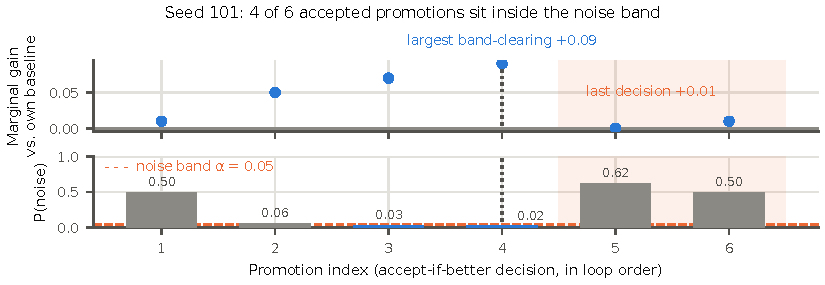
\includegraphics[width=0.96\linewidth]{../figures/exp4_stopping_seed101.pdf}
  % source figure (generated by `mdi report`, do not edit):
  %   exp4_stopping_seed101.pdf <- data/derived/exp4/promotions.json
  %   (rows + stopping[] for seed 101, alpha=0.05)
  \caption{Regimes seed 101: held-out gain per accepted decision against its
    noise probability. Four of the six do not clear the $\alpha{=}0.05$ band;
    the largest that clears is \#4 ($+0.09$), and the two taken after it
    measure $+0.00$ and $+0.01$.}
  \label{fig:loop-remeasure}
\end{figure}

\section{A Reporting-and-Decision Protocol}
\label{sec:protocol}

Reporting prescriptions exist (TEE's checklist \citep{messing2026tee}, NIST AI
800-3's repeat-trial minimum \citep{nist2026ai8003}), but not the decision
rule that turns reported uncertainty into a licensed claim. The protocol below
adds that step and nothing more.

When reporting an improvement measured by an LLM judge:
\begin{enumerate}
  \item \textbf{Repeat}: score with $N \geq 3$ independent repeats per
    system in the stated environment.
  \item \textbf{Interval}: report a confidence interval for the gain
    $\Delta$, not a point estimate alone.
  \item \textbf{Decide}: claim only when $\Delta > \mdi_{\alpha}(\env, N)$
    \emph{on the stated item set} \textbf{and} $\fip(\Delta, \env, N) \leq
    \alpha$. The first is a pre-experimental threshold, the second prices the
    gain actually observed; a $\Delta$ just past $\mdi$ can still reverse a
    quarter of the time (Table~\ref{tab:fip-conversion}).
\end{enumerate}
Steps 2 and 3 are both necessary: a gain clearing $\mdi$ whose interval still
covers zero is not licensed.
The two enter at different times: $\mdi$ before the run, to choose the $N$
a target gain requires, and $\fip$ after it, to price the gain observed.
Since the $\fip$ read-off exceeds $\mdi$ in every cell of our grid
(Section~\ref{sec:exp1}), it is usually the $\fip$ condition that binds.
$\fip$ costs no second evaluation: it is estimated from the same repeated
scoring that yields $\mdi$, with repeat~$0$ held out as the screening pass
(Experiment~2), and a team reads its own environment's row off the resulting
conversion table (Table~\ref{tab:fip-conversion}) instead of recomputing one
per decision. None of the three speaks to where the
instrument is aimed (Section~\ref{sec:limitations}). The protocol fixes the \emph{rule}, not a
universal threshold; no constant survives even our own grid, and the
hand-picked ones the loop of Section~\ref{sec:exp4} shipped (a $0.0$ default,
a $+0.02$ remedy) sit below its measured band. %
Measuring your own costs under
\$0.20 per system (dense) or \$10.38 (anchor) at $N{=}20$ over $100$ items;
an $A$-vs-$B$ pair is twice that (Table~\ref{tab:cost}).

\paragraph{Absolute decisions: the SLA margin table.}
The rule above is relative ($A$ vs.\ $B$); delivery decisions are often
absolute, and the same null distribution prices a contract threshold $t$ too
(Table~\ref{tab:sla-margin}): G-theory's absolute/relative distinction
\citep{cronbach1972dependability, messing2026tee}.
Every entry is \emph{fixed-prompt}, and Section~\ref{sec:exp3}'s shared prompt
component exceeds every margin in the table
(Appendix~\ref{app:extra}): re-wording a rubric moves an absolute score by more
than the margin it must clear. Re-calibrate rather than reuse.



Every number in this paper passes all three steps, traceable to a derived
record and a run identifier.

\section{Limitations}
\label{sec:limitations}

\paragraph{Consistency, not validity.}
Everything we measure is test--retest consistency, and
Section~\ref{sec:experiments} measures the size of the gap against the
benchmark's expert annotations rather than asserting it. $\mdi$ and $\fip$
license a claim \emph{as scored by this judge}, not one about what it should
score, and a finer threshold makes a mis-aimed instrument more confident,
not more correct.

\paragraph{Low noise is necessary, not sufficient.}
Clearing $\mdi(\env, N)$ rules out the instability channel only: a gain can
clear it and still be judge \emph{bias} \citep{zhou2026selfplay}, which repeats
do not average away. Experiment~3 separates the channels but removes neither
bias nor the floor's own uncertainty: we wrote the paraphrases (all eight are
in Appendix~\ref{app:paraphrases}), and the four added second raised it
$2.5\times$. The first four proved
unrepresentatively alike; ours may be unrepresentatively varied. We report the
dependence, not a value.

\paragraph{Our $\sigma$ is a lower bound on production variability.}
The systems are frozen, so every wobble is the judge's and agent-side variance
is a separate environment (Section~\ref{sec:framework}). Three narrower
caveats: null pools sit inside one system, valid for $A$-vs-$B$ only under
comparable spread ($1.32\times$ at the widest); both judges share a provider,
leaving Section~\ref{sec:exp1}'s reversal attributable to scale or stack; and
item sampling is out of scope, so $\mdi$ licenses a claim about the stated
item set, not the population.
The grid is narrow in kind as well as size: two text tasks, one provider,
temperature~$1$ throughout, and no agent traces, so the agent pipelines that
motivate the question are argued from, not measured.



\bibliographystyle{plainnat}
\bibliography{references}

\appendix

\section{Additional Tables and Diagnostics}
\label{app:extra}

\begin{table}[h]
  \centering
  \caption{SLA margin: to claim ``score $\geq t$'', the observed $N$-repeat mean
    must exceed $t$ by the cell value [\%p; $\sigma$-relative in parentheses],
    the one-sided $95\%$ null quantile per environment. Read off the null
    \emph{difference} distribution, it prices the uncertainty in $t$ as well,
    so against an exactly known $t$ every entry is conservative by $\sqrt{2}$.
    Section~\ref{sec:exp3}'s shared prompt component, $6.83$~\%p, is
    $2.7$--$12\times$ the $N{=}1$ column ($0.55$--$2.50$~\%p) and
    $2.7$--$25\times$ this whole table ($0.27$--$2.50$~\%p).
    Pilot estimates.}
  \label{tab:sla-margin}
  \scriptsize
  \renewcommand{\arraystretch}{0.88}
  % sla_margin.tex — generated by `mdi report tables`; DO NOT hand-edit.
% One-sided 95% absolute-claim margin in %p: claim `score >= t` only when
% the observed N-repeat mean exceeds t by at least the cell value
% (sigma-relative in parentheses). Read-off of the alpha=0.10 null entry's
% |delta| 0.90-quantile (decision record 015, 2026-08-02).
% Provenance:
%   exp1_alpaca: run_ids [r_20260801_44f551, r_20260801_cc2370]  sha256:3d28470d4c85e824c9649789ffaad27919b8db63dcce4ddd6fc439220b8526cf
%   exp1_anchor: run_ids [r_20260801_0eeb4b, r_20260801_856cc9]  sha256:e7e21136aed59136fc840db08a3e1635d26871f7850d8677c914a56a366ee464
%   exp1_anchor_scales: run_ids [r_20260801_011dec, r_20260801_8133fe]  sha256:fa348c3e7f1acba0b8410630139efcc911382006c2a6c2e0522e6af6148f98b8
%   exp1_dense: run_ids [r_20260801_45dffd, r_20260801_da6e9c]  sha256:bd8102f54e78061a856b434d33b565be50c857875483ff205a9f124d18ae5303
\begin{tabular*}{\linewidth}{@{\extracolsep{\fill}}lcccc}
  \toprule
  & \multicolumn{4}{c}{Margin over $t$ [\%p]} \\
  \cmidrule(lr){2-5}
  Environment & $N{=}1$ & $N{=}3$ & $N{=}5$ & $N{=}8$ \\
  \midrule
  4o-mini $\cdot$ Summ $\cdot$ L5 & 1.50 (0.23$\sigma$) & 0.92 (0.14$\sigma$) & 0.80 (0.12$\sigma$) & 0.69 (0.11$\sigma$) \\  % e_250190cb1b81
  gpt-5.6 $\cdot$ Summ $\cdot$ L5 & 2.50 (0.35$\sigma$) & 1.67 (0.23$\sigma$) & 1.60 (0.22$\sigma$) & -- \\  % e_b842cbff3261
  4o-mini $\cdot$ Summ $\cdot$ L10 & 1.11 (0.24$\sigma$) & 0.67 (0.14$\sigma$) & 0.56 (0.12$\sigma$) & 0.50 (0.11$\sigma$) \\  % e_7268666f4d91
  4o-mini $\cdot$ Summ $\cdot$ S100 & 0.90 (0.24$\sigma$) & 0.56 (0.15$\sigma$) & 0.45 (0.12$\sigma$) & 0.41 (0.11$\sigma$) \\  % e_200f3c74cbfa
  gpt-5.6 $\cdot$ Summ $\cdot$ S100 & 1.05 (0.37$\sigma$) & -- & 0.69 (0.24$\sigma$) & -- \\  % e_d26d4476fba5
  4o-mini $\cdot$ Instr $\cdot$ L5 & 1.00 (0.23$\sigma$) & 0.58 (0.14$\sigma$) & 0.50 (0.12$\sigma$) & 0.44 (0.10$\sigma$) \\  % e_dabfcd0d96e0
  4o-mini $\cdot$ Instr $\cdot$ L10 & 0.89 (0.23$\sigma$) & 0.56 (0.14$\sigma$) & 0.47 (0.12$\sigma$) & 0.42 (0.11$\sigma$) \\  % e_9dae315a7446
  4o-mini $\cdot$ Instr $\cdot$ S100 & 0.55 (0.22$\sigma$) & 0.38 (0.15$\sigma$) & 0.32 (0.13$\sigma$) & 0.27 (0.11$\sigma$) \\  % e_1cfecd45841e
  \bottomrule
\end{tabular*}

\end{table}

\begin{table}[t]
  \centering
  \caption{Noise-floor decomposition (Experiment~3 environment): total SD
    of the $N$-mean, observed vs.\ the no-floor $1/\sqrt{N}$ extrapolation
    of the $N{=}1$ spread, in \%p (raw in parentheses). $N \in \{1,3,5\}$
    measured; $N{=}20$, $N{\to}\infty$ from the fit (Eq.~\ref{eq:decay}).
    The last row is the same cell swept over four paraphrases instead of
    eight. Pilot estimates.}
  \label{tab:noise-floor}%
  %% source: data/derived/exp3_decay8/decay.json (fits[0].points sd_mean,
  %% sd_theoretical for N in {1,3,5}; sigma_sq, omega_sq, omega for the
  %% model columns). run_ids r_20260805_5b3342 (pilot), r_20260805_523960;
  %% env_id e_e941458fd533. Observed N=20 = sqrt(sigma_sq/20 + omega_sq),
  %% N=inf = omega; both /4*100 to %p. Four-paraphrase row: same quantities
  %% from data/derived/exp3_decay/decay.json, env_id e_a7cb4136ad0c.
  \footnotesize
  \begin{tabular*}{\linewidth}{@{\extracolsep{\fill}}lccccc}
    \toprule
    Total SD of $N$-mean [\%p (raw)]
      & $N{=}1$ & $N{=}3$ & $N{=}5$ & $N{=}20$ & $N{\to}\infty$ \\
    \midrule
    Observed (with floor $\omega$)
      & 10.26 (0.411) & 9.12 (0.365) & 8.86 (0.354) & 8.58 (0.343) & 8.48 (0.339) \\
    No-floor $1/\sqrt{N}$
      & 10.26 (0.411) & 5.93 (0.237) & 4.59 (0.184) & 2.30 (0.092) & 0 (0) \\
    \midrule
    Same cell, four paraphrases
      & 7.90 (0.316) & 6.31 (0.252) & 5.91 (0.236) & 5.47 (0.219) & 5.31 (0.213) \\
    \bottomrule
  \end{tabular*}
\end{table}


\begin{figure}[h]
  \centering
  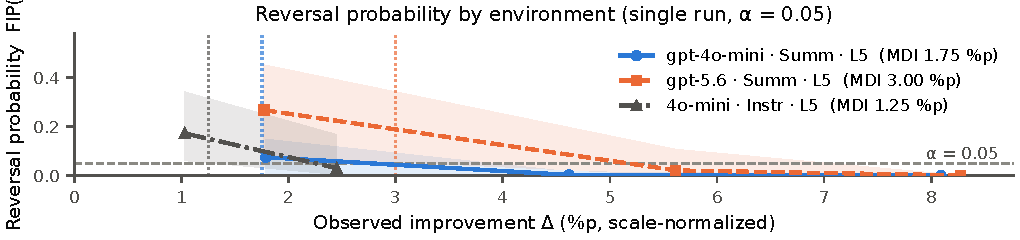
\includegraphics[width=\linewidth]{../figures/fip_overlay_N1_alpha0p05.pdf}
  % source figure (generated by `mdi report`, do not edit):
  %   fip_overlay_N1_alpha0p05.pdf -- the three headline envs on one axes,
  %   selection fixed in figures.HEADLINE_FIP_ENVS.
  %   run_ids: dense r_20260801_da6e9c, anchor r_20260801_0eeb4b,
  %   alpaca r_20260801_cc2370
  \caption{Reversal probability against observed gain at $N{=}1$ (bootstrap
    95\% CIs, cluster $=$ system pair; dotted verticals mark each
    environment's $\mdi$). Near-pair reversal is $7.4\%$ for dense
    \texttt{gpt-4o-mini} against $26.7\%$ for anchor \texttt{gpt-5.6} on the
    same cell, and $17.2\%$ on instruction-following. The judge contrast's
    intervals overlap; the ordering is a point-estimate statement.}
  \label{fig:fip-curves}
\end{figure}

\paragraph{Conversion table (Experiment 2).}
The full observed-gain $\rightarrow$ reversal-probability conversion, whose
headline contrast (the same $1.8$~\%p gain reversing $7.4\%$ under
\texttt{gpt-4o-mini} but $26.7\%$ under \texttt{gpt-5.6}) appears in
Section~\ref{sec:exp2}, is Table~\ref{tab:fip-conversion}.

\begin{table}[h]
  \centering
  \caption{Conversion table: a single-run observed gain $\rightarrow$
    estimated reversal probability, per environment (lowest $\Delta$ bin,
    $N{=}1$; $\fip$ with bootstrap 95\% CI). The same $\Delta$ carries
    different risk in different environments.}
  \label{tab:fip-conversion}
  %% source: paper/tables/fip_conversion.csv (N=1 rows, first bin per env);
  %% equivalently data/derived/{exp1_dense,exp1_anchor,exp1_alpaca}/fip.json.
  \small
  \begin{tabular*}{\linewidth}{@{\extracolsep{\fill}}lcc}
    \toprule
    Environment (judge $\cdot$ task $\cdot$ scale)
      & Observed $\Delta$ [\%p (raw)]
      & $\fip(\Delta,\env,1)$ [\%, CI] \\
    \midrule
    gpt-5.6 $\cdot$ Summ $\cdot$ L5   & $1.8$ (0.071) & 26.7 [8.1, 45.2] \\
    4o-mini $\cdot$ Summ $\cdot$ L5   & $1.8$ (0.072) & 7.4 [0.0, 14.8] \\
    4o-mini $\cdot$ Summ $\cdot$ L10  & $1.5$ (0.135) & 1.5 [0.0, 2.6] \\
    4o-mini $\cdot$ Summ $\cdot$ S100 & $1.1$ (1.064) & 6.7 [0.0, 10.9] \\
    4o-mini $\cdot$ Instr $\cdot$ L5  & $1.0$ (0.041) & 17.2 [6.0, 34.1] \\
    4o-mini $\cdot$ Instr $\cdot$ L10 & $0.8$ (0.071) & 20.3 [9.4, 32.3] \\
    4o-mini $\cdot$ Instr $\cdot$ S100 & $0.6$ (0.550) & 27.5 [9.9, 42.3] \\
    \bottomrule
  \end{tabular*}
\end{table}

\paragraph{Near-pair FIP against repeats (Experiment 2).}
Dense summarization clears near-pair reversals by $N{=}5$
($7.4 \rightarrow 0.5\%$), but the anchor and AlpacaEval environments stay in
double digits even at $N{=}10$ (anchor likert5 $26.7 \rightarrow 10.2\%$;
instruction score100 $27.5 \rightarrow 14.2\%$).
%% source: paper/tables/fip_conversion.csv, first-bin reversal_pct at
%% n_repeats in {1,5,10} for each env. (likert10/likert5
%% instruction decay figures remain in the csv.)

\paragraph{Decay of the $N$-repeat mean (Experiment 3).}
Measured SD of the $N$-mean against the no-floor $1/\sqrt{N}$ reference, over
the \emph{four}-paraphrase family of the dense
summarization~$\times$~likert5 environment (the last row of
Table~\ref{tab:noise-floor}). The fit (Eq.~\ref{eq:decay}; $\sigma^2 = 0.055$,
$\omega^2 = 0.045$) resolves a floor that averaging cannot cross; the
eight-paraphrase family of the same cell flattens onto $8.48$~\%p instead
(Section~\ref{sec:exp3}).

\begin{figure}[h]
  \centering
  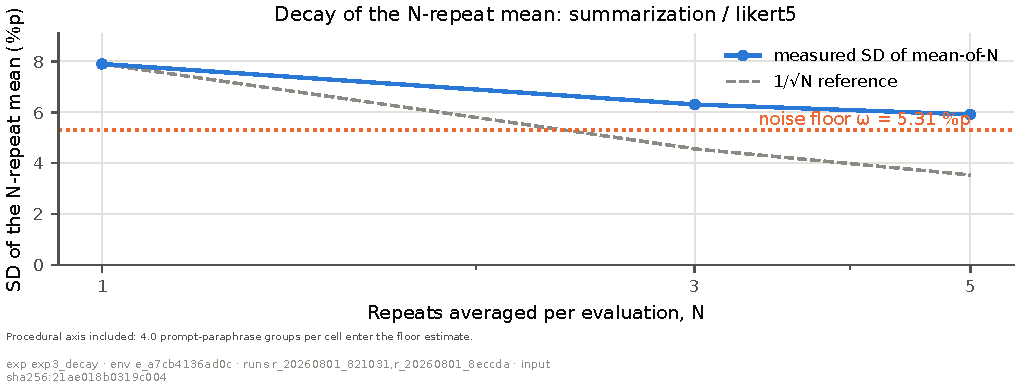
\includegraphics[width=\linewidth]{../figures/decay_curve_exp3_decay_e_a7cb4136ad0c.pdf}
  % source figure (generated by `mdi report`, do not edit):
  %   run_ids r_20260801_821031, r_20260801_8eccda; env_id e_a7cb4136ad0c
  \caption{Decay of the $N$-repeat mean over the \emph{four}-paraphrase family
    of the dense summarization~$\times$~likert5 cell (the last row of
    Table~\ref{tab:noise-floor}), drawn at $\omega = 5.31$~\%p. The measured
    curve flattens onto $\omega$ while the no-floor $1/\sqrt{N}$ reference
    keeps falling; widening the family to eight moves the same cell's floor to
    $8.48$~\%p (Section~\ref{sec:exp3}).}
  \label{fig:decay-curves}
\end{figure}

\paragraph{Consistency check, per-cell numbers (Experiment 1).}
At $N{=}1$, summarization likert5 gives null-PI $1.75$ vs.\ FIP-crossing
$2.74$~\%p ($\times 1.56$) for \texttt{gpt-4o-mini} and $3.00$ vs.\ $5.15$~\%p
($\times 1.72$) for \texttt{gpt-5.6}; the full per-cell comparison is the
\texttt{consistency} block of each environment's \texttt{mdi\_table.json}. The gap is
systematic (the FIP read-off is always larger) because the sustained-crossing
rule prices in a stricter criterion than the raw null half-width; it is a
disclosed property of the two estimators, not an error.
%% source: data/derived/exp1_*/mdi_table.json ("consistency" block).

\paragraph{Sweep-truncation mechanics (Experiment 1, caveat i).}
The null distribution draws two disjoint pools per cell, but the draws inside
each pool are taken \emph{with replacement}, so the split does not itself bound
$N$: a budget larger than a pool can be simulated. What bounds the lookup is a
reporting rule: an $N$ is kept only when \emph{every} cell holds at least $N$
estimation repeats, because reporting simulated budgets would overstate what the
data measured. Every cell holds 19 estimation repeats in the dense and alpaca
tiers (20 raw, repeat~0 held out for screening) and 7 in the anchor, so the rule
leaves no $N{=}20$ entry anywhere on the null-PI path and stops the anchor at
$N{=}5$. The quantifier is load-bearing: a \emph{some}-cell rule would open the
anchor's $N{=}8$ column on the strength of one cell in 200 that holds an eighth
repeat, while the other 199 could only simulate that budget. The FIP path shares
the same draw machinery but applies no such truncation, and therefore reaches
$N{=}10$ on the anchor.

\paragraph{Estimation-pool inflation.}
The two null pools are a split of a cell's $r$ estimation repeats, so their means
differ by a split-half term that no budget removes. Writing
$P = \tfrac{1}{|A|} + \tfrac{1}{|B|}$ for the two pools ($|A| + |B| = r$, so
$P \approx 4/r$), one item contributes
$\sigma^2\bigl[(2 - P)/N + P\bigr]$: the within-pool part loses $P/N$ because a
pool of size $a$ has population variance $\sigma^2(a{-}1)/a$, and the pools' own
means differ by $\sigma^2 P$. The reported half-width is therefore
\[
  \mdi_{\alpha}(\env, N) \;\approx\;
  \frac{z_{1-\alpha/2}\,\sigma}{\sqrt{|I|}}
  \sqrt{\tfrac{2 - P}{N} + P},
\]
rather than $z_{1-\alpha/2}\sigma\sqrt{2/N}/\sqrt{|I|}$, the value for an
unlimited pool. Two consequences. At $N{=}1$ the two terms cancel \emph{exactly}
(one draw from each pool is just two draws from the $r$ repeats), so there is
no inflation at all; and the excess grows with the budget, reaching $39.6\%$ at
$N{=}10$ on $r{=}19$ and $47.2\%$ at $N{=}5$ on $r{=}7$
(Table~\ref{tab:pool-inflation}). In the dense
summarization~$\times$~likert5 cell ($\sigma = 6.40$~\%p, $|I| = 100$, pools of
$9$ and $10$) the model gives $1.77, 1.13, 0.94, 0.83, 0.78$~\%p against the
measured $1.75, 1.13, 0.93, 0.84, 0.78$, within $2\%$ everywhere, where the
$2/N + P$ form this appendix previously quoted was high by up to $7\%$. The
inflation is conservative, demanding
a larger gain than the instability alone requires, and it is largest where $r$ is
smallest: it is the second reason the anchor tier carries no large-$N$ column, and
the reason MDI is not compared across tiers with different $r$. The corrected
column is released beside the raw one in the derived records; the archival grid
will report MDI at matched $r$.

\begin{table}[h]
  \centering
  \caption{What the estimator adds on top of the environment. The factor is
    $\sqrt{[(2-P)/N + P] \big/ (2/N)}$ for the split this project's repeat counts
    produce; the corrected row divides it out of the dense
    summarization~$\times$~likert5 cell. At $N{=}1$ the split costs nothing.}
  \label{tab:pool-inflation}
  %% source: data/derived/exp1_*/mdi_table.json null_entries[].pool_inflation
  %% and .mdi_null_corrected_pp (alpha=0.05). Verified against a direct
  %% simulation of the draw procedure.
  \footnotesize
  \begin{tabular*}{\linewidth}{@{\extracolsep{\fill}}lccccc}
    \toprule
    & $N{=}1$ & $N{=}3$ & $N{=}5$ & $N{=}8$ & $N{=}10$ \\
    \midrule
    Dense / instruction tiers ($r{=}19$, pools $9{+}10$)
      & $1.000$ & $1.101$ & $1.193$ & $1.319$ & $1.396$ \\
    Anchor tier ($r{=}7$, pools $3{+}4$)
      & $1.000$ & $1.258$ & $1.472$ & -- & -- \\
    \midrule
    4o-mini $\cdot$ Summ $\cdot$ L5, as reported [\%p]
      & 1.75 & 1.13 & 0.93 & 0.84 & 0.78 \\
    \quad corrected [\%p]
      & 1.75 & 1.02 & 0.78 & 0.64 & 0.55 \\
    \bottomrule
  \end{tabular*}
\end{table}

\paragraph{The external reference, per pair (Experiment 1).}
The SummEval release annotates every summarizer on four facets with three
experts; the pair-selection step reads them to choose the closest four systems, and
Section~\ref{sec:exp1} reads them again to check the instrument. Over the $100$
scored items the four differ by at most $1.15$~\%p and no pair of the six has an
interval excluding zero, so the set is externally null: a null this paper's
estimator did not construct, which is what makes the coverage below
non-circular. The reference is itself a measurement: its widest pair interval is
$4.52$~\%p, so ``not separated'' means ``not separated at this precision'',
never ``identical''. Averaged over the six pairs, $|$judge gap$|$ is
$4.54$~\%p against $|$reference gap$|$ $0.57$~\%p in the likert5 cell, leaving
$4.73$~\%p unaccounted for; the residual does not shrink with $N$.
One environment reverses this. On \texttt{gpt-5.6}~$\cdot$~score100 the judge
spread is $2.07$~\%p against the reference's $1.67$, and agreement is $0.67$,
so the unaccounted residual is a property of the environment, not a fact about
judges as a class.
%% source: data/derived/exp1_anchor_scales/oracle.json reports[].{judge_spread_pp,
%% oracle_spread_pp, rank_concordance}; env gpt-5.6 x summarization x score100.

\begin{table}[h]
  \centering
  \caption{Claim rate against the two nulls, dense
    summarization~$\times$~likert5. \emph{Internal} re-scores one system twice
    (the channel $\mdi$ is built to control); it lands at the two-sided $\alpha$ where
    the pool term vanishes ($N{=}1$) and below it thereafter, the same artifact
    Table~\ref{tab:pool-inflation} prices. \emph{External} compares two systems
    the reference cannot separate. Both rows are two-sided $|\Delta|$
    readings; the directional rule of Section~\ref{sec:protocol} fires at
    half the internal row. Only the first is a property of the threshold.}
  \label{tab:oracle-coverage}
  %% source: data/derived/exp1_dense/oracle.json reports[env=e_250190cb1b81]
  %% .claim_rates[] (alpha=0.05, 200 draws per pair, 6 pairs / 4 systems).
  \footnotesize
  \begin{tabular*}{\linewidth}{@{\extracolsep{\fill}}lccccc}
    \toprule
    & $N{=}1$ & $N{=}3$ & $N{=}5$ & $N{=}8$ & $N{=}10$ \\
    \midrule
    $\mdi_{.05}$ [\%p]           & 1.75  & 1.13  & 0.93  & 0.84  & 0.78 \\
    Internal null (one system)   & 0.043 & 0.028 & 0.018 & 0.007 & 0.004 \\
    External null (unseparated pairs) & 0.829 & 0.934 & 0.960 & 0.983 & 0.993 \\
    \bottomrule
  \end{tabular*}
\end{table}
%% source: data/derived/exp1_{dense,anchor}/mdi_table.json meta.params
%% .estimation_repeats; support rule = src/mdi/stats/null_mdi.py supported_sweep
%%. Pool term = 1/|A| + 1/|B| for the split of r; dense 1/9+1/10=0.211.

\paragraph{The known-effect ladder (Experiment 1 validation pass).}
The eleven-system pass behind Section~\ref{sec:exp1}'s boundary numbers spans
external gaps of $0.00$--$37.02$~\%p over the same $100$ items and the same
environment as the dense likert5 cell (registry: \texttt{exp1\_ladder}).
Detection is the share of scoring draws with $|\Delta| > \mdi(\env, N)$,
computed with the same draw machinery as the claim rates below.
Pooled over the ten pairs the reference cannot separate, the claim rate rises
$0.878 \to 0.999$ from $N{=}1$ to $N{=}10$ while the internal rate falls
$0.034 \to 0.008$; the per-pair detection curves, the per-facet separation
flags behind the ``no facet / three of four'' sentences, and the two boundary
summaries are recorded fields of the derived record.
%% source: data/derived/exp1_ladder/oracle.json reports[env=e_250190cb1b81]
%% .{claim_rates[].{internal,external}_rate, detection[], detection_summary[],
%% facet_reports[], gaps[].facets_separating}; runs r_20260814_2f48e2 (pilot)
%% + r_20260814_c8104e (full), config 41ff28672647ee0c.

\paragraph{Held-out screening: scope note (Experiment 2).}
Pair selection separates a screening pass (repeat~0) from FIP estimation, and
the guard fires on intentional overlap (it raises
when the screening and estimation repeat indices intersect); all held-out runs
pass it. On this data, held-out did not
measurably move FIP: held-out vs.\ no-holdout estimates differ on the order of
$\pm 0.1$--$2.6$~\%p with mixed signs. The reason is structural rather than a
null result: the current FIP estimation path bins \emph{all}
system pairs by re-observed $\Delta$ rather than pre-selecting close pairs on
the screening $\Delta$, so excluding repeat~0 removes only one of
$\sim$19--20 estimation repeats and the selection-on-noise inflation the
held-out design targets is never exercised. The guard remains a required safeguard for a
future close-pair pre-selection analysis; here it is enforced but
structurally inert.
%% source: docs/papers/EXP2-fip-results.md sec.4 (held-out vs no-holdout
%% comparison) + sec.1 (OverlappingRepeatsError guard demonstration).

\paragraph{Per-system spread (heteroscedasticity check).}
$\mdi$ builds its null distribution inside one system and averages over
systems, which represents an $A$-vs-$B$ comparison only if the systems have
comparable spread. They do: across all eight environments the widest
system-to-system ratio is $1.32$, and it is $1.10$--$1.24$ in five of the eight.
The same requirement is why judges are compared by $\sigma$, which is
item-count-independent, and never by $\mdi$: the anchor cells use fewer items,
so their $\mdi$ is not on the dense tier's footing.

\begin{table}[h]
  \centering
  \caption{Repeat instability per system within each environment, in \%p
    (pooled over items, estimation repeats only). ``ratio'' is the widest
    system divided by the narrowest; a large value would mean the null
    distribution is centred on the wrong variance.}
  \label{tab:system-sigma}
  %% source: data/derived/exp1_*/variance.json, "systems" rows (
  %% 2026-08-06). sigma in %p = raw / scale-width * 100.
  \footnotesize
  \begin{tabular*}{\linewidth}{@{\extracolsep{\fill}}lccc}
    \toprule
    Environment (judge $\cdot$ task $\cdot$ scale)
      & narrowest $\sigma$ & widest $\sigma$ & ratio \\
    \midrule
    4o-mini $\cdot$ Summ $\cdot$ L5    & 5.46 & 7.18 & 1.32 \\
    4o-mini $\cdot$ Instr $\cdot$ L10  & 3.32 & 4.28 & 1.29 \\
    4o-mini $\cdot$ Instr $\cdot$ S100 & 2.18 & 2.69 & 1.24 \\
    4o-mini $\cdot$ Instr $\cdot$ L5   & 3.77 & 4.54 & 1.21 \\
    gpt-5.6 $\cdot$ Summ $\cdot$ L5    & 6.55 & 7.82 & 1.19 \\
    gpt-5.6 $\cdot$ Summ $\cdot$ S100  & 2.73 & 3.07 & 1.12 \\
    4o-mini $\cdot$ Summ $\cdot$ S100  & 3.56 & 3.94 & 1.11 \\
    4o-mini $\cdot$ Summ $\cdot$ L10   & 4.53 & 5.01 & 1.10 \\
    \bottomrule
  \end{tabular*}
\end{table}

\paragraph{Null-pair construction (estimand and estimator).}
For an environment $\env$, let $R_{s,i}$ be the estimation repeats of
system $s$ on item $i$, and let $\bar{m}_N(P)$ denote the mean of $N$
scores drawn with replacement from a pool $P$. One null draw for system
$s$ is
\begin{equation*}
  \delta_s^{(b)}
    \;=\; \frac{1}{|I|} \sum_{i \in I}
      \Bigl( \bar{m}_N\bigl(A^{(b)}_{s,i}\bigr)
            - \bar{m}_N\bigl(B^{(b)}_{s,i}\bigr) \Bigr),
\end{equation*}
where $(A^{(b)}_{s,i}, B^{(b)}_{s,i})$ is a fresh uniform partition of
$R_{s,i}$ into disjoint pools, drawn independently per item and per draw
$b$. Both pools score the same cell, so the true difference is zero by
construction, and the pairing is at the \emph{item} level: system-level
means enter only through the average over $I$, never through cross-system
differencing. Pooling $\delta_s^{(b)}$ over systems and draws gives the
empirical $D_0(\env, N)$; $\mdi$ is the half-width of its central
interval, and the confidence interval on $\mdi$ is a seeded cluster
bootstrap over systems (all draws of one system resampled together).
Relative CI width on the reported $\mdi$ runs $4.3$--$30.6\%$ (median
$14.3\%$ over the $35$ published cells); with four system clusters the usual
$(G{-}1)/G$ bias applies, so we read it as a spread rather than calibrated
coverage.

\paragraph{Family-wise correction (Experiment 4).}
The band of Section~\ref{sec:experiments} is applied per decision. Under a
Holm--Bonferroni correction across all $14$ promotion $p$-values (family
$\alpha = 0.05$), exactly one promotion remains individually significant:
seed~$5$'s $11$-vs-$1$ ($p = 0.0032$); seed~$101$'s promotions $3$--$4$
($p = 0.033$, $0.025$) do not survive. The seed-$101$ diagnosis is unaffected
in direction: its $7$-vs-$6$ last accepted decision is a failure to clear
the band, which stricter control only reinforces, and a family-wise gate would have promoted
nothing on that seed. The per-decision band is an operating policy, not a
family-wise inference. The McNemar null further treats a promotion's $n$
discordant answers as independent fair-coin flips, which correlated failure
modes across questions would violate.
%% source: data/derived/exp4/promotions.json rows[].reversal_prob, Holm
%% step-down at alpha=0.05 over m=14; survivor = seed 5 promo #4 (11,1).

%% source: data/derived/exp4/promotions.json rows[].confirm_baseline_acc
%% (seed 101), computed from the release's own confirm_baseline_outcomes.
\paragraph{The prospective bar (Experiment 4).}
The band is computable \emph{before} a loop runs: at discordant counts of
the size this loop produced, the smallest gain that would clear
$\alpha{=}0.05$ is $+0.06$ to $+0.09$, above both constants the loop shipped
(Section~\ref{sec:protocol}).
%% source: prospective_min_delta over n in [7,17] (src/mdi/stats/promotion.py).

\paragraph{Marginals, not a trajectory (Experiment 4).}
Each accepted decision is scored against the state in force when it was taken,
and on seed~$101$ those states differ: the six \texttt{confirm} baselines are
$0.79$, $0.80$, $0.80$, $0.77$, $0.80$ and $0.78$ on the same $100$ held-out
questions. The six gains are therefore marginals against six different
baselines, so no ordering of them is a trajectory and summing them would not
describe where the loop finished.

\paragraph{Statistical notes.}
(1)~$\mdi_{\alpha}$ is parameterized by $\alpha$ through the central
$(1-\alpha)$ interval; $\alpha$ is two-sided throughout, events are read
as $|\Delta|$, and $\fip$ alone is one-sided, a signed reversal probability.
The decision rule of Section~\ref{sec:protocol} claims only positive gains,
so its false-claim rate under the null is $\alpha/2$; in the dense summarization~$\times$~likert5 cell
at $N{=}1$ $\mdi_{\alpha}$ is $1.50$~\%p at $\alpha{=}0.10$ and $2.38$~\%p at
$\alpha{=}0.01$, against $1.75$~\%p at the headline $\alpha{=}0.05$.
(2)~FIP confidence intervals are cluster-bootstrapped at the system-pair
level (six pairs), the coarsest available unit; coarse clustering widens the
interval while six clusters bias it low, so we report it as a spread rather
than calibrated coverage.
(3)~The \%p normalization eases cross-scale reading, but the underlying
scale widths differ ($4$, $9$, $100$ points), so raw-scale values are
carried alongside throughout (parentheses in the body,
Table~\ref{tab:raw-sigma} in full).
(4)~The measured $80\%$ factor of Section~\ref{sec:framework} matches the
$1+z_{1-\beta}/z_{1-\alpha/2}$ a normal $D_0$ would give and recovers the
$(z_{1-\alpha/2}{+}z_{1-\beta})$ form used on the item axis
\citep{kotawala2026resolution}, so the approximation is a checked choice.

\section{Reproducibility Details}
\label{app:repro}

Every judge call was issued by the framework's runner (\texttt{mdi run})
through an \texttt{mdi estimate-cost}~$\rightarrow$~pilot~$\rightarrow$~full
gate, logged to an
append-only ledger, and stored with a content-addressed input snapshot;
analyses are seeded and sorted, and regenerating every figure and table
twice produces byte-identical files. The code, the configuration files, the
raw scores and the derived records (everything needed to re-run the
analyses and reproduce every figure and table) are available at
\url{https://github.com/wigtn/mdi-artifact}.
Judges are \texttt{gpt-4o-mini}
(dense tier) and \texttt{gpt-5.6} (anchor tier; \texttt{max\_completion\_tokens}
interface) via the OpenAI API, temperature $1.0$, runs of 2026-08-01/02 and 2026-08-05.
Experiment~3 distributes forty repeats per cell round-robin over eight
prompt paraphrases sharing one environment id. Experiment~4 issues no API
calls: it is computed from the public Regimes release
(\texttt{github.com/yoheinakajima/regimes}, Apache-2.0, commit
\texttt{7ba11a9}) pinned under the input snapshot store, derived record
digest \texttt{sha256:01a90e87c48c\ldots}.
A tied re-measurement counts as a reversal, which inflates
$\fip$ on coarse scales and is therefore conservative for a claim.

\begin{table}[h]
  \centering
  \caption{Measured cost in USD per $100$ (item~$\times$~system) cells at
    budget $N$, per judge tier: ledger spend over logged calls,
    $\times\,N \times 100$. Because the ledger aggregates pilot and full
    passes, the per-tier unit price mixes their call counts; the anchor
    column therefore differs from a direct division of
    Table~\ref{tab:run-registry} by about $0.2\%$. Pilot scale; generated from
    the ledger by \texttt{mdi report} (digest in the file header).}
  \label{tab:cost}
  \footnotesize
  % cost_table.tex — generated by `mdi report tables`; DO NOT hand-edit.
% Measured USD per 100 (item x system) cells at N scoring
% repeats: ledger total spend / total calls per judge tier, x N x 100.
% Provenance: data/ledger.jsonl sha256:59b588c8f0eb
%   dense: 48001 calls, $4.4142 logged
%   anchor: 2891 calls, $14.9987 logged
%   skipped (no derived tier mapping): exp1_ladder, exp3_decay, exp3_decay8, spike_fip, spike_fip_gpt56
\begin{tabular*}{\linewidth}{@{\extracolsep{\fill}}lcccc}
  \toprule
  & \multicolumn{4}{c}{USD per 100 cells} \\
  \cmidrule(lr){2-5}
  Judge tier & $N{=}1$ & $N{=}3$ & $N{=}8$ & $N{=}20$ \\
  \midrule
  dense & 0.009 & 0.028 & 0.074 & 0.184 \\
  anchor & 0.519 & 1.556 & 4.150 & 10.376 \\
  \bottomrule
\end{tabular*}

\end{table}

\begin{table}[h]
  \centering
  \caption{Run registry (full-grid runs). The counts are full-run
    aggregates only; the complementary pilot passes (sharing these config
    hashes in the same ledger) complete the nominal cell product, with a
    handful of parse-failure retries above it. $^{*}$Raising the repeats per
    cell changes the config hash, so the eight-paraphrase environment took a
    second gated pass; the runner is idempotent on
    (env, item, system, repeat), so it billed only the $6{,}400$ new calls and
    the two rows plus this environment's $120$-call pilot sum to the
    $16{,}000$ records Section~\ref{sec:exp3} reports.}
  \label{tab:run-registry}
  %% source: data/ledger.jsonl, aggregated per run_id (spike runs excluded).
  \footnotesize
  \begin{tabular*}{\linewidth}{@{\extracolsep{\fill}}llllrr}
    \toprule
    Experiment & run\_id & config hash & input digest & calls & USD \\
    \midrule
    exp1\_dense         & r\_20260801\_da6e9c & 57230b2ac56a5ffe & c04b5053f276 & 23{,}640 & 2.27 \\
    exp1\_alpaca        & r\_20260801\_cc2370 & 6455906059207bcb & 716ce514f138 & 23{,}641 & 2.09 \\
    exp1\_anchor        & r\_20260801\_0eeb4b & 471dabd1861b8f7a & 1f69dfca06f0 & 1{,}569  & 7.50 \\
    exp1\_anchor\_scales & r\_20260801\_8133fe & e52338b922a693b2 & d12fd21c8be9 & 1{,}242  & 7.11 \\
    exp1\_ladder        & r\_20260814\_c8104e & 41ff28672647ee0c & ac908ce9c639 & 21{,}670 & 2.09 \\
    exp3\_decay         & r\_20260801\_8eccda & 97a5b1d31c9b8385 & c04b5053f276 & 7{,}880  & 0.76 \\
    exp3\_decay8        & r\_20260805\_a9d7a3 & 1abfa882321f4392 & c04b5053f276 & 9{,}480  & 0.91 \\
    exp3\_decay8$^{*}$  & r\_20260805\_523960 & 07f436c4afaa217e & c04b5053f276 & 6{,}400  & 0.62 \\
    \bottomrule
  \end{tabular*}
\end{table}

\begin{table}[h]
  \centering
  \caption{Raw-scale repeat instability per environment (raw values live
    here by convention; the body reports \%p $=$ raw~/~scale
    width~$\times 100$). Bootstrap 95\% CIs, cluster $=$ item.}
  \label{tab:raw-sigma}
  %% source: paper/tables/variance_by_env.csv (sigma, sigma_ci_lo/hi).
  \footnotesize
  \begin{tabular*}{\linewidth}{@{\extracolsep{\fill}}llll}
    \toprule
    Environment & env\_id & raw $\sigma$ [95\% CI] & $\sigma$ [\%p] \\
    \midrule
    4o-mini $\cdot$ Summ $\cdot$ L5    & e\_250190cb1b81 & 0.2560 [0.2375, 0.2734] & 6.40 \\
    gpt-5.6 $\cdot$ Summ $\cdot$ L5    & e\_b842cbff3261 & 0.2860 [0.2530, 0.3157] & 7.15 \\
    4o-mini $\cdot$ Summ $\cdot$ L10   & e\_7268666f4d91 & 0.4219 [0.4089, 0.4347] & 4.69 \\
    4o-mini $\cdot$ Summ $\cdot$ S100  & e\_200f3c74cbfa & 3.8159 [3.6222, 3.9979] & 3.82 \\
    gpt-5.6 $\cdot$ Summ $\cdot$ S100  & e\_d26d4476fba5 & 2.8558 [2.7024, 3.0087] & 2.86 \\
    4o-mini $\cdot$ Instr $\cdot$ L5   & e\_dabfcd0d96e0 & 0.1712 [0.1364, 0.2030] & 4.28 \\
    4o-mini $\cdot$ Instr $\cdot$ L10  & e\_9dae315a7446 & 0.3453 [0.3079, 0.3831] & 3.84 \\
    4o-mini $\cdot$ Instr $\cdot$ S100 & e\_1cfecd45841e & 2.4651 [2.1254, 2.8314] & 2.47 \\
    \bottomrule
  \end{tabular*}
\end{table}

\section{Experiment 3 Rubric Paraphrases}
\label{app:paraphrases}
The eight templates behind Section~\ref{sec:exp3}'s floor, verbatim, so the
family can be judged directly rather than through its variance.
\texttt{\{\{source\}\}} and \texttt{\{\{candidate\}\}} mark where the article
and the summary are inserted; line breaks are joined. All eight hold the four
criteria, the $1$--$5$ scale and the JSON reply contract fixed and vary wording
only. The first four are the family behind the four-paraphrase floor of
$5.31$~\%p (the last row of Table~\ref{tab:noise-floor}); the full eight give
$8.48$~\%p. Experiment~1's summarization~$\times$~likert5 cells, both judges
and the validation pass, are scored with \texttt{pp\_0}'s wording.

\noindent\texttt{pp\_0} \emph{(four-paraphrase family)}
\begin{quote}\small
You are evaluating the quality of a summary. \\
Read the source article and the candidate summary, then rate the summary's overall quality on a 1-5 scale, where 1 is very poor and 5 is excellent. Consider relevance, coherence, fluency, and factual consistency with the source. \\
Source article: \texttt{\{\{source\}\}} \\
Candidate summary: \texttt{\{\{candidate\}\}} \\
Reply with JSON and nothing else, in exactly this form: \texttt{\{"score": <integer 1-5>\}}
\end{quote}
\noindent\texttt{pp\_1} \emph{(four-paraphrase family)}
\begin{quote}\small
Your task is to judge how good a summary is. \\
Below are a source article and a summary written from it. Assign an overall quality rating between 1 and 5, where 1 means very poor and 5 means excellent. Base your judgment on how relevant the summary is, how coherent it reads, how fluent it is, and how factually faithful it stays to the source. \\
Article: \texttt{\{\{source\}\}} \\
Summary to rate: \texttt{\{\{candidate\}\}} \\
Return only JSON, exactly like this: \texttt{\{"score": <integer 1-5>\}}
\end{quote}
\noindent\texttt{pp\_2} \emph{(four-paraphrase family)}
\begin{quote}\small
Act as an evaluator of summary quality. \\
Given the original article and a candidate summary, provide a single overall score from 1 (very poor) to 5 (excellent). Weigh four things: whether the summary is relevant, whether it reads coherently, whether it is fluent, and whether it remains factually consistent with the article. \\
Original article: \texttt{\{\{source\}\}} \\
Candidate summary: \texttt{\{\{candidate\}\}} \\
Respond with JSON only, in precisely this format: \texttt{\{"score": <integer 1-5>\}}
\end{quote}
\noindent\texttt{pp\_3} \emph{(four-paraphrase family)}
\begin{quote}\small
You will score the quality of a summary. \\
After reading the source text and the proposed summary, rate the summary overall on a scale from 1 to 5 (1 = very poor, 5 = excellent). Take into account its relevance, its coherence, its fluency, and its factual agreement with the source text. \\
Source text: \texttt{\{\{source\}\}} \\
Proposed summary: \texttt{\{\{candidate\}\}} \\
Answer with JSON and nothing more, exactly in this shape: \texttt{\{"score": <integer 1-5>\}}
\end{quote}
\noindent\texttt{pp\_4}
\begin{quote}\small
Rate the summary below. \\
You are given an article and a summary of it. Give one overall rating from 1 to 5, with 1 the worst and 5 the best. Four things should inform the rating: relevance, coherence, fluency, and factual consistency with the article. \\
Article: \texttt{\{\{source\}\}} \\
Summary: \texttt{\{\{candidate\}\}} \\
Output JSON only, exactly: \texttt{\{"score": <integer 1-5>\}}
\end{quote}
\noindent\texttt{pp\_5}
\begin{quote}\small
How good is this summary? \\
Read the source below, then the summary written from it. Decide on a single overall quality score in the range 1-5 (1 = very poor, 5 = excellent). Ask yourself about its relevance, its coherence, its fluency, and its factual consistency with the source. \\
Source: \texttt{\{\{source\}\}} \\
Summary: \texttt{\{\{candidate\}\}} \\
Give your answer as JSON and nothing else: \texttt{\{"score": <integer 1-5>\}}
\end{quote}
\noindent\texttt{pp\_6}
\begin{quote}\small
You are a summary quality assessor. \\
Assess the candidate summary against the source article and report one overall score between 1 and 5, where 1 denotes very poor quality and 5 denotes excellent quality. The assessment covers four criteria: (1) relevance, (2) coherence, (3) fluency, (4) factual consistency with the article. \\
Article text: \texttt{\{\{source\}\}} \\
Summary under assessment: \texttt{\{\{candidate\}\}} \\
Your reply must be JSON only, in this exact form: \texttt{\{"score": <integer 1-5>\}}
\end{quote}
\noindent\texttt{pp\_7}
\begin{quote}\small
Score a summary for overall quality. \\
The source article comes first, then a summary of it. Produce one overall score on a five-point scale where 1 is very poor and 5 is excellent, judged on relevance, coherence, fluency, and factual agreement with the source. \\
The article: \texttt{\{\{source\}\}} \\
Its summary: \texttt{\{\{candidate\}\}} \\
Reply with nothing but JSON, in this exact shape: \texttt{\{"score": <integer 1-5>\}}
\end{quote}

\end{document}
